\documentclass[11pt]{article}
\usepackage[margin=2cm]{geometry}
\usepackage{amsmath,amssymb,amsthm}
\usepackage{tikz}
\usetikzlibrary{calc,arrows.meta,positioning,decorations.pathreplacing,backgrounds,shapes.geometric}
\usepackage{caption}

\newcommand{\Sv}{\mathrm{S}_v}
\newcommand{\Qt}{\widetilde{Q}}

% Shared styles
\tikzset{
  vtx/.style={circle, fill=blue!70, inner sep=1.8pt},
  pvtx/.style={circle, fill=magenta!80, inner sep=1.8pt},
  svtx/.style={circle, fill=red!70, inner sep=1.8pt},
  dnode/.style={circle, draw, thick, fill=white, minimum size=16pt, font=\scriptsize},
  snode/.style={circle, draw, thick, fill=cyan!20, minimum size=16pt, font=\scriptsize},
  pnode/.style={rectangle, draw, thick, fill=green!15, minimum size=14pt, font=\scriptsize, rounded corners=2pt},
  ann/.style={draw, rounded corners=3pt, fill=white, font=\scriptsize, align=left, inner sep=4pt},
  fbox/.style={draw, thick, rounded corners=3pt, minimum height=1cm, align=center, font=\small},
}

\begin{document}

\section*{Diagrams for Section 2: A strong $d$-step theorem for spindles}

%% =============================================
%% DEFINITION 2.1
%% =============================================
\subsection*{Definition 2.1 --- Dual steps and the dual Hirsch conjecture}

\begin{figure}[h]
\centering
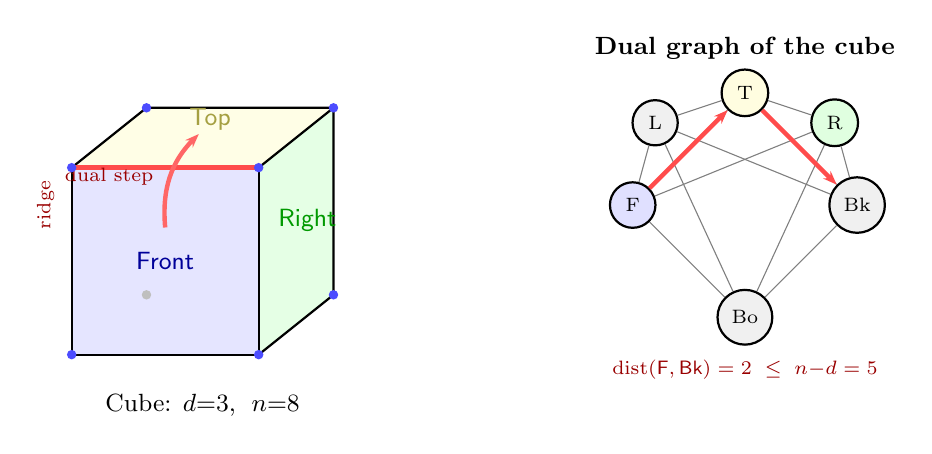
\begin{tikzpicture}[scale=0.95]
  % --- Cube ---
  \begin{scope}[shift={(-4.5,0)}]
    % Front face
    \coordinate (A1) at (0,0);
    \coordinate (B1) at (2.5,0);
    \coordinate (C1) at (2.5,2.5);
    \coordinate (D1) at (0,2.5);
    % Back face
    \coordinate (A2) at (1,0.8);
    \coordinate (B2) at (3.5,0.8);
    \coordinate (C2) at (3.5,3.3);
    \coordinate (D2) at (1,3.3);

    % Hidden edges
    \draw[thick, dashed, gray!50] (A1)--(A2);
    \draw[thick, dashed, gray!50] (A2)--(B2);
    \draw[thick, dashed, gray!50] (A2)--(D2);

    % Visible faces
    \fill[blue!10] (A1)--(B1)--(C1)--(D1)--cycle;
    \fill[green!10] (B1)--(B2)--(C2)--(C1)--cycle;
    \fill[yellow!10] (D1)--(C1)--(C2)--(D2)--cycle;

    % Visible edges
    \draw[thick] (A1)--(B1)--(C1)--(D1)--cycle;
    \draw[thick] (B1)--(B2)--(C2)--(C1);
    \draw[thick] (D1)--(D2)--(C2);

    % Ridge (shared edge Front--Top)
    \draw[ultra thick, red!70] (D1)--(C1);
    \node[font=\scriptsize, red!60!black, rotate=90] at (-0.35,2.0) {ridge};

    % Face labels
    \node[font=\small, blue!60!black] at (1.25,1.25) {\textsf{Front}};
    \node[font=\small, green!60!black] at (3.15,1.8) {\textsf{Right}};
    \node[font=\small, yellow!60!black] at (1.85,3.15) {\textsf{Top}};

    % Dual-step arrow between facet centers
    \draw[-{Stealth[length=5pt]}, ultra thick, red!60, bend left=25]
      (1.25,1.7) to node[left=2pt, font=\scriptsize, red!60!black] {dual step} (1.7,2.95);

    % Vertices
    \foreach \p in {A1,B1,C1,D1,B2,C2,D2}
      \fill[blue!70] (\p) circle (1.8pt);
    \fill[gray!50] (A2) circle (1.8pt);

    \node[below, font=\small] at (1.75,-0.4) {Cube: $d{=}3$,\; $n{=}8$};
  \end{scope}

  % --- Dual graph ---
  \begin{scope}[shift={(3,0.5)}]
    \node[font=\bfseries\small] at (1.5,3.6) {Dual graph of the cube};

    \node[dnode, fill=blue!12] (Fr) at (0,1.5) {F};
    \node[dnode, fill=gray!12] (Bk) at (3,1.5) {Bk};
    \node[dnode, fill=yellow!12] (T) at (1.5,3) {T};
    \node[dnode, fill=gray!12] (Bo) at (1.5,0) {Bo};
    \node[dnode, fill=green!12] (R) at (2.7,2.6) {R};
    \node[dnode, fill=gray!12] (L) at (0.3,2.6) {L};

    % Edges (gray)
    \draw[gray] (Fr)--(Bo)--(Bk)--(T)--(Fr);
    \draw[gray] (Fr)--(R)--(Bk);
    \draw[gray] (Fr)--(L)--(Bk);
    \draw[gray] (T)--(R)--(Bo)--(L)--(T);

    % Highlighted shortest path F -> T -> Bk
    \draw[-{Stealth[length=5pt]}, ultra thick, red!70] (Fr)--(T);
    \draw[-{Stealth[length=5pt]}, ultra thick, red!70] (T)--(Bk);

    \node[font=\scriptsize, red!60!black] at (1.5,-0.7) {$\mathrm{dist}(\textsf{F},\textsf{Bk}) = 2 \;\leq\; n{-}d = 5$};
  \end{scope}
\end{tikzpicture}
\caption*{\textbf{Definition 2.1:} A $d$-polytope $Q$ with $n$ vertices is \emph{dual-Hirsch}
if $n - d$ dual steps suffice to travel between any two facets.
A \emph{dual step} moves from a facet $F$ to an adjacent facet $F'$ across a shared
\emph{ridge} (codimension-2 face). The dual Hirsch conjecture is equivalent to the
primal one via polarity.}
\end{figure}


%% =============================================
%% LEMMA 2.2 — 3D pushing: facets increase
%% =============================================
\subsection*{Lemma 2.2 --- Pushing a vertex (3D: facets can split)}

\begin{figure}[h]
\centering
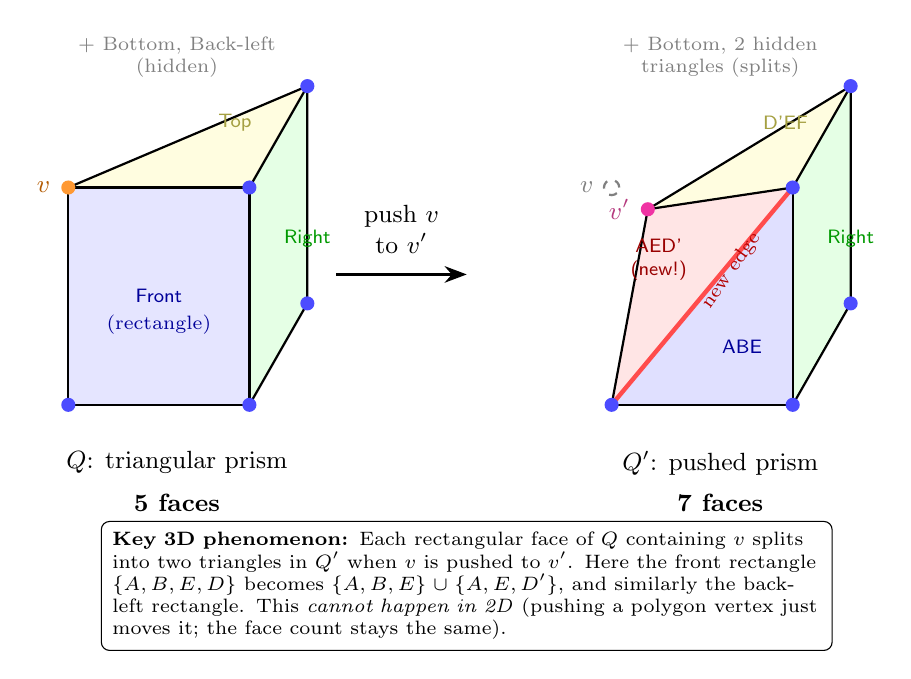
\begin{tikzpicture}[scale=0.92]
  %% === Original prism Q (left) ===
  \begin{scope}[shift={(-5,0)}]
    % Bottom triangle
    \coordinate (A) at (0,0);
    \coordinate (B) at (2.5,0);
    \coordinate (C) at (3.3,1.4);
    % Top triangle
    \coordinate (D) at (0,3);
    \coordinate (E) at (2.5,3);
    \coordinate (F) at (3.3,4.4);

    % Hidden edge
    \draw[thick, dashed, gray!50] (A)--(C);

    % Fill visible faces
    \fill[blue!10] (A)--(B)--(E)--(D)--cycle;        % Front
    \fill[green!10] (B)--(C)--(F)--(E)--cycle;       % Right
    \fill[yellow!12] (D)--(E)--(F)--cycle;            % Top

    % Draw edges
    \draw[thick] (A)--(B)--(E)--(D)--cycle;           % Front
    \draw[thick] (B)--(C)--(F)--(E);                  % Right
    \draw[thick] (D)--(F);                             % Top back edge
    \draw[thick] (C)--(F);

    % Face labels
    \node[font=\scriptsize, blue!60!black] at (1.25,1.5) {\textsf{Front}};
    \node[font=\scriptsize, blue!60!black] at (1.25,1.1) {(rectangle)};
    \node[font=\scriptsize, green!60!black] at (3.3,2.3) {\textsf{Right}};
    \node[font=\scriptsize, yellow!60!black] at (2.3,3.9) {\textsf{Top}};

    % Highlight vertex D
    \foreach \p in {A,B,C,E,F} \node[vtx] at (\p) {};
    \node[vtx, fill=orange!80] at (D) {};
    \node[left=3pt, font=\small, orange!70!black] at (D) {$v$};

    % Hidden faces label
    \node[font=\scriptsize, gray, align=center] at (1.5,4.8) {+ Bottom, Back-left\\(hidden)};

    \node[font=\small, below] at (1.5,-0.5) {$Q$: triangular prism};
    \node[font=\bfseries\small, below] at (1.5,-1.1) {5 faces};
  \end{scope}

  % Arrow
  \draw[-{Stealth[length=8pt]}, thick] (-1.3,1.8) -- (0.5,1.8)
    node[midway, above=4pt, font=\small, align=center] {push $v$\\to $v'$};

  %% === Pushed prism Q' (right) ===
  \begin{scope}[shift={(2.5,0)}]
    % Same bottom
    \coordinate (A) at (0,0);
    \coordinate (B) at (2.5,0);
    \coordinate (C) at (3.3,1.4);
    % Pushed vertex
    \coordinate (Dp) at (0.5,2.7);   % D' pushed inside
    \coordinate (E) at (2.5,3);
    \coordinate (F) at (3.3,4.4);

    % Hidden edges
    \draw[thick, dashed, gray!50] (A)--(C);
    \draw[thick, dashed, gray!50] (A)--(F);  % new edge (hidden, splits back-left)

    % Fill: front face SPLIT into two triangles
    \fill[blue!12] (A)--(B)--(E)--cycle;              % Lower triangle
    \fill[red!10] (A)--(E)--(Dp)--cycle;              % Upper triangle (NEW)

    % Fill: right face unchanged
    \fill[green!10] (B)--(C)--(F)--(E)--cycle;

    % Fill: top face (tilted)
    \fill[yellow!12] (Dp)--(E)--(F)--cycle;

    % Draw edges
    \draw[thick] (A)--(B)--(E);
    \draw[thick] (A)--(Dp)--(E);
    \draw[thick] (B)--(C)--(F)--(E);
    \draw[thick] (Dp)--(F);

    % Splitting diagonal — the key new edge
    \draw[ultra thick, red!70] (A)--(E);

    % Ghost of old vertex D
    \draw[dashed, gray, thick] (0,3) circle (3pt);
    \node[left=3pt, font=\small, gray] at (0,3) {$v$};

    % Face labels
    \node[font=\scriptsize, blue!60!black] at (1.8,0.8) {\textsf{ABE}};
    \node[font=\scriptsize, red!60!black] at (0.65,2.2) {\textsf{AED'}};
    \node[font=\scriptsize, red!60!black] at (0.65,1.85) {\textsf{(new!)}};
    \node[font=\scriptsize, green!60!black] at (3.3,2.3) {\textsf{Right}};
    \node[font=\scriptsize, yellow!60!black] at (2.4,3.9) {\textsf{D'EF}};

    % Vertices
    \foreach \p in {A,B,C,E,F} \node[vtx] at (\p) {};
    \node[pvtx] at (Dp) {};
    \node[left=3pt, font=\small, magenta!70!black] at (Dp) {$v'$};

    % New edge label
    \node[font=\scriptsize, red!70!black, rotate=55] at (1.65,1.85) {new edge};

    \node[font=\scriptsize, gray, align=center] at (1.5,4.8) {+ Bottom, 2 hidden\\triangles (splits)};
    \node[font=\small, below] at (1.5,-0.5) {$Q'$: pushed prism};
    \node[font=\bfseries\small, below] at (1.5,-1.1) {7 faces};
  \end{scope}

  % Annotation box
  \node[ann, text width=9cm] at (0.5,-2.5) {%
    \textbf{Key 3D phenomenon:} Each rectangular face of $Q$ containing $v$
    splits into two triangles in $Q'$ when $v$ is pushed to $v'$.
    Here the front rectangle $\{A,B,E,D\}$ becomes $\{A,B,E\} \cup \{A,E,D'\}$,
    and similarly the back-left rectangle. This \emph{cannot happen in 2D}
    (pushing a polygon vertex just moves it; the face count stays the same).};
\end{tikzpicture}
\caption*{\textbf{Lemma 2.2 (3D illustration):} Pushing $v$ to $v'$ in a triangular prism.
The two rectangles containing $v$ each split into two triangles (5 faces $\to$ 7 faces).
The map $\phi$ sends each facet of $Q'$ to the unique facet of $Q$ containing its vertex
set (minus the $v \leftrightarrow v'$ swap). Multiple facets of $Q'$ can map to the same facet of $Q$.}
\end{figure}

\newpage

%% =============================================
%% LEMMA 2.2 — Proof: continuous deformation
%% =============================================
\subsection*{Lemma 2.2 --- Proof (continuous deformation and the simplicial map $\phi$)}

\begin{figure}[h]
\centering
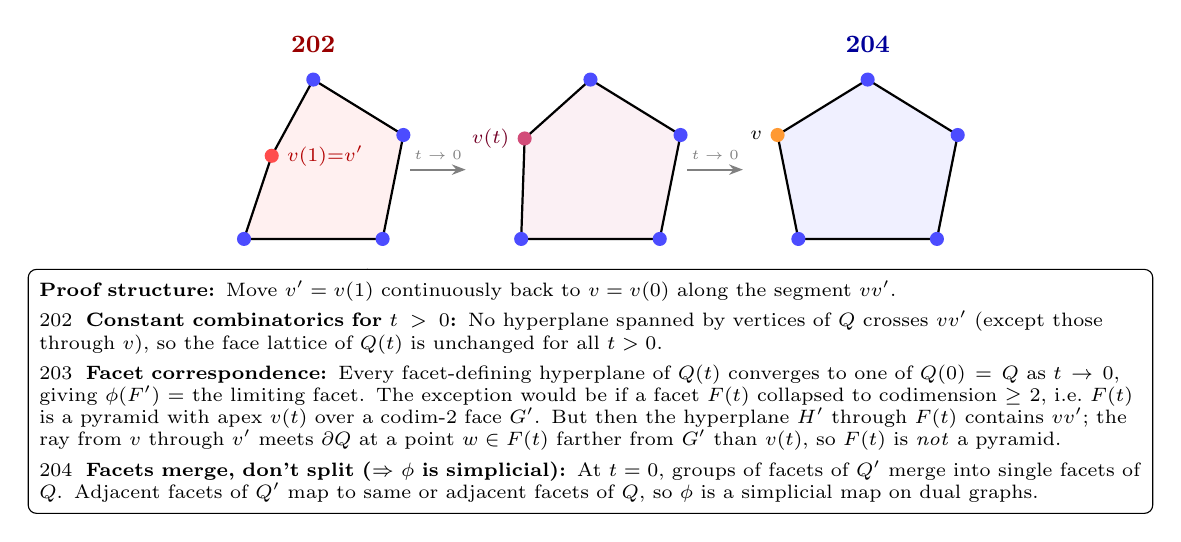
\begin{tikzpicture}[scale=0.88]
  %% t=1: Q(1) = Q'
  \begin{scope}[shift={(-5.5,0)}]
    \coordinate (A) at (0,0);
    \coordinate (B) at (2,0);
    \coordinate (C) at (2.3,1.5);
    \coordinate (D) at (1,2.3);
    \coordinate (V1) at (0.4,1.2);
    \fill[red!6] (A)--(B)--(C)--(D)--(V1)--cycle;
    \draw[thick] (A)--(B)--(C)--(D)--(V1)--cycle;
    \foreach \p in {A,B,C,D} \node[vtx] at (\p) {};
    \node[svtx] at (V1) {};
    \node[right=2pt, font=\scriptsize, red!70!black] at (V1) {$v(1){=}v'$};
    \node[below, font=\small] at (1,-0.3) {$Q(1) = Q'$};
    % Circled 1
    \node[font=\bfseries\small, red!60!black] at (1,2.8) {\ding{202}};
  \end{scope}

  \draw[-{Stealth[length=5pt]}, thick, gray] (-3.1,1) -- (-2.3,1)
    node[midway, above, font=\tiny] {$t \to 0$};

  %% t in (0,1): Q(t) — same combinatorics
  \begin{scope}[shift={(-1.5,0)}]
    \coordinate (A) at (0,0);
    \coordinate (B) at (2,0);
    \coordinate (C) at (2.3,1.5);
    \coordinate (D) at (1,2.3);
    \coordinate (V2) at (0.05,1.45);
    \fill[purple!6] (A)--(B)--(C)--(D)--(V2)--cycle;
    \draw[thick] (A)--(B)--(C)--(D)--(V2)--cycle;
    \foreach \p in {A,B,C,D} \node[vtx] at (\p) {};
    \node[circle, fill=purple!70, inner sep=1.8pt] at (V2) {};
    \node[left=2pt, font=\scriptsize, purple!60!black] at (V2) {$v(t)$};
    \node[below, font=\small] at (1,-0.3) {$Q(t)$, $t \in (0,1)$};
  \end{scope}

  \draw[-{Stealth[length=5pt]}, thick, gray] (0.9,1) -- (1.7,1)
    node[midway, above, font=\tiny] {$t \to 0$};

  %% t=0: Q(0) = Q — facets merge
  \begin{scope}[shift={(2.5,0)}]
    \coordinate (A) at (0,0);
    \coordinate (B) at (2,0);
    \coordinate (C) at (2.3,1.5);
    \coordinate (D) at (1,2.3);
    \coordinate (V0) at (-0.3,1.5);
    \fill[blue!6] (A)--(B)--(C)--(D)--(V0)--cycle;
    \draw[thick] (A)--(B)--(C)--(D)--(V0)--cycle;
    \foreach \p in {A,B,C,D} \node[vtx] at (\p) {};
    \node[vtx, fill=orange!80] at (V0) {};
    \node[left=2pt, font=\scriptsize] at (V0) {$v$};
    \node[below, font=\small] at (1,-0.3) {$Q(0) = Q$};
    % Circled 3
    \node[font=\bfseries\small, blue!60!black] at (1,2.8) {\ding{204}};
  \end{scope}

  %% Proof annotations below
  \node[ann, text width=14cm] at (-0.5,-2.2) {%
    \textbf{Proof structure:}
    Move $v' = v(1)$ continuously back to $v = v(0)$ along the segment $vv'$.\\[3pt]
    \ding{202}\; \textbf{Constant combinatorics for $t > 0$:}
    No hyperplane spanned by vertices of $Q$ crosses $vv'$ (except those through $v$),
    so the face lattice of $Q(t)$ is unchanged for all $t > 0$.\\[3pt]
    \ding{203}\; \textbf{Facet correspondence:}
    Every facet-defining hyperplane of $Q(t)$ converges to one of $Q(0) = Q$ as $t \to 0$,
    giving $\phi(F') = $ the limiting facet. The exception would be if a facet $F(t)$ collapsed
    to codimension $\geq 2$, i.e.\ $F(t)$ is a pyramid with apex $v(t)$ over a codim-2 face $G'$.
    But then the hyperplane $H'$ through $F(t)$ contains $vv'$; the ray from $v$ through $v'$
    meets $\partial Q$ at a point $w \in F(t)$ farther from $G'$ than $v(t)$, so $F(t)$ is \emph{not} a pyramid. \;$\lightning$\\[3pt]
    \ding{204}\; \textbf{Facets merge, don't split ($\Rightarrow$ $\phi$ is simplicial):}
    At $t = 0$, groups of facets of $Q'$ merge into single facets of $Q$.
    Adjacent facets of $Q'$ map to same or adjacent facets of $Q$, so $\phi$ is a simplicial map on dual graphs.
  };
\end{tikzpicture}
\caption*{\textbf{Lemma 2.2, proof:}
The assumption $v' \in Q$ (not just the interior) is essential to rule out pyramid collapse.}
\end{figure}


%% =============================================
%% LEMMA 2.2 — Simplicial map on dual graphs
%% =============================================
\begin{figure}[h]
\centering
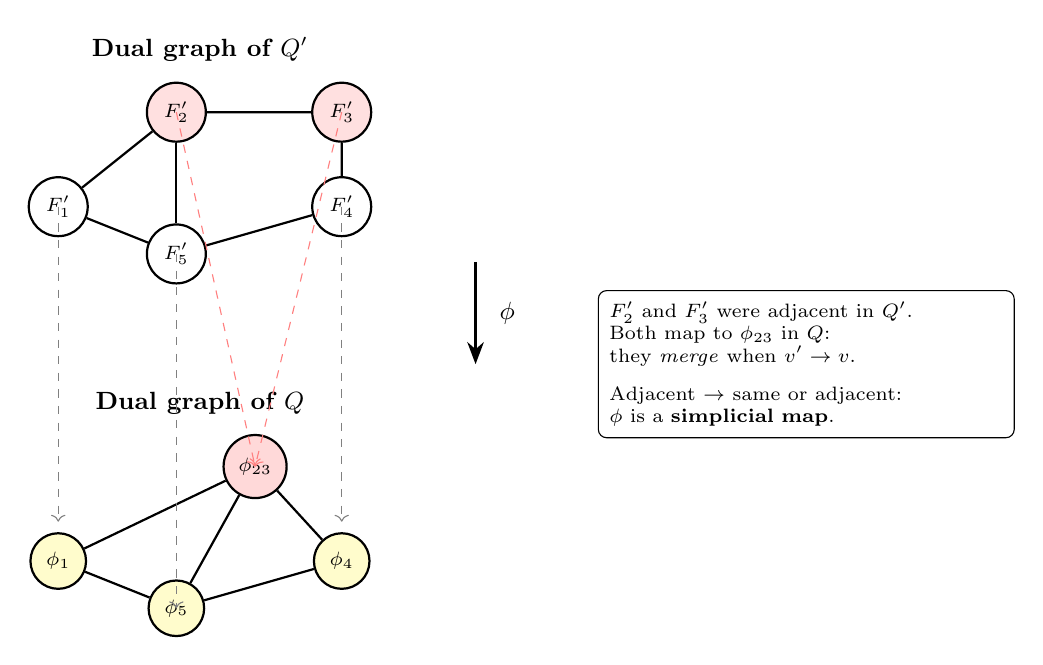
\begin{tikzpicture}[scale=1.0]
  % --- Dual graph of Q' ---
  \begin{scope}[shift={(-4,2.5)}]
    \node[font=\bfseries\small] at (1.8,2) {Dual graph of $Q'$};
    \node[dnode] (F1) at (0,0) {$F'_1$};
    \node[dnode, fill=red!12] (F2) at (1.5,1.2) {$F'_2$};
    \node[dnode, fill=red!12] (F3) at (3.6,1.2) {$F'_3$};
    \node[dnode] (F4) at (3.6,0) {$F'_4$};
    \node[dnode] (F5) at (1.5,-0.6) {$F'_5$};
    \draw[thick] (F1)--(F2)--(F3)--(F4)--(F5)--(F1);
    \draw[thick] (F2)--(F5);
  \end{scope}

  % Phi arrow
  \draw[-{Stealth[length=8pt]}, thick] (1.3,1.8) -- (1.3,0.5)
    node[midway, right=5pt, font=\small] {$\phi$};

  % --- Dual graph of Q ---
  \begin{scope}[shift={(-4,-2)}]
    \node[font=\bfseries\small] at (1.8,2) {Dual graph of $Q$};
    \node[dnode, fill=yellow!20] (G1) at (0,0) {$\phi_1$};
    \node[dnode, fill=red!15] (G23) at (2.5,1.2) {$\phi_{23}$};
    \node[dnode, fill=yellow!20] (G4) at (3.6,0) {$\phi_4$};
    \node[dnode, fill=yellow!20] (G5) at (1.5,-0.6) {$\phi_5$};
    \draw[thick] (G1)--(G23)--(G4)--(G5)--(G1);
    \draw[thick] (G23)--(G5);
  \end{scope}

  % Mapping arrows
  \draw[->, dashed, gray] (-4,2.5) -- (-4,-1.5);
  \draw[->, dashed, red!50] (-2.5,3.7) -- (-1.5,-0.8);
  \draw[->, dashed, red!50] (-0.4,3.7) -- (-1.5,-0.8);
  \draw[->, dashed, gray] (-0.4,2.5) -- (-0.4,-1.5);
  \draw[->, dashed, gray] (-2.5,1.9) -- (-2.5,-2.6);

  % Annotation
  \node[ann, text width=5cm] at (5.5,0.5) {%
    $F'_2$ and $F'_3$ were adjacent in $Q'$.\\
    Both map to $\phi_{23}$ in $Q$:\\
    they \emph{merge} when $v' \to v$.\\[6pt]
    Adjacent $\to$ same or adjacent:\\
    $\phi$ is a \textbf{simplicial map}.
  };
\end{tikzpicture}
\caption*{\textbf{Lemma 2.2, part (2):}
The map $\phi\colon F' \mapsto \phi(F')$ sends adjacent facets of $Q'$ to the same
or adjacent facets of $Q$. \textbf{Corollary 2.3 (Klee):} For every polytope $Q$,
there is a \emph{simplicial} polytope $Q'$ with the same dimension and number of
vertices and the same or greater dual diameter. (Push all non-simple vertices.)}
\end{figure}

\newpage

%% =============================================
%% LEMMA 2.4 — Dual graph projection
%% =============================================
\subsection*{Lemma 2.4 --- One-point-suspension preserves dual distances}

\begin{figure}[h]
\centering
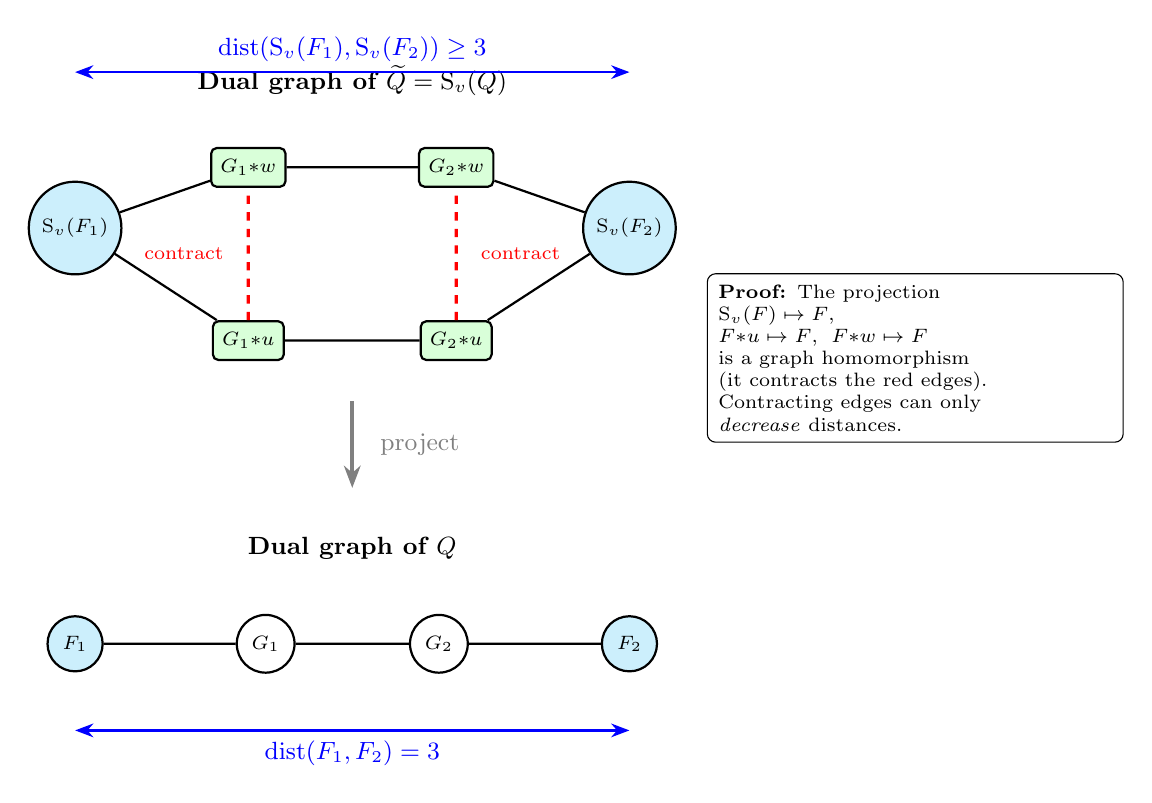
\begin{tikzpicture}[scale=1.1]
  % --- Top: Dual graph of S_v(Q) ---
  \node[font=\bfseries\small] at (0,5.2) {Dual graph of $\Qt = \Sv(Q)$};

  \node[snode] (SvF1) at (-3.2,3.5) {$\Sv(F_1)$};
  \node[snode] (SvF2) at (3.2,3.5) {$\Sv(F_2)$};

  \node[pnode] (G1u) at (-1.2,2.2) {$G_1{\ast}u$};
  \node[pnode] (G1w) at (-1.2,4.2) {$G_1{\ast}w$};
  \node[pnode] (G2u) at (1.2,2.2) {$G_2{\ast}u$};
  \node[pnode] (G2w) at (1.2,4.2) {$G_2{\ast}w$};

  % Dual edges
  \draw[thick] (SvF1)--(G1u);
  \draw[thick] (SvF1)--(G1w);
  \draw[thick] (G1u)--(G2u);
  \draw[thick] (G1w)--(G2w);
  \draw[thick] (G2u)--(SvF2);
  \draw[thick] (G2w)--(SvF2);

  % Contractible edges (red dashed)
  \draw[very thick, red, dashed] (G1u)--(G1w)
    node[midway, left=5pt, font=\scriptsize, red] {contract};
  \draw[very thick, red, dashed] (G2u)--(G2w)
    node[midway, right=5pt, font=\scriptsize, red] {contract};

  % Projection arrow
  \draw[-{Stealth[length=8pt]}, ultra thick, gray] (0,1.5) -- (0,0.5)
    node[midway, right=6pt, font=\small] {project};

  % --- Bottom: Dual graph of Q ---
  \node[font=\bfseries\small] at (0,-0.2) {Dual graph of $Q$};

  \node[snode] (F1) at (-3.2,-1.3) {$F_1$};
  \node[dnode] (G1) at (-1,-1.3) {$G_1$};
  \node[dnode] (G2) at (1,-1.3) {$G_2$};
  \node[snode] (F2) at (3.2,-1.3) {$F_2$};

  \draw[thick] (F1)--(G1)--(G2)--(F2);

  % Distance labels
  \draw[{Stealth}-{Stealth}, thick, blue] (-3.2,-2.3)--(3.2,-2.3)
    node[midway, below, font=\small, blue] {$\mathrm{dist}(F_1, F_2) = 3$};
  \draw[{Stealth}-{Stealth}, thick, blue] (-3.2,5.3)--(3.2,5.3)
    node[midway, above, font=\small, blue] {$\mathrm{dist}(\Sv(F_1), \Sv(F_2)) \geq 3$};

  % Proof annotation
  \node[ann, text width=5cm] at (6.5,2) {%
    \textbf{Proof:} The projection\\
    $\Sv(F) \mapsto F$,\\
    $F{\ast}u \mapsto F$,\;
    $F{\ast}w \mapsto F$\\
    is a graph homomorphism\\
    (it contracts the red edges).\\
    Contracting edges can only\\
    \emph{decrease} distances.
  };
\end{tikzpicture}
\caption*{\textbf{Lemma 2.4:}
Facets of $\Sv(Q)$: if $v \in F$, the facet is $\Sv(F)$; if $v \notin F$,
the facet splits into two pyramids $F{\ast}u$ and $F{\ast}w$.
The dual graph of $\Sv(Q)$ surjects onto that of $Q$ by contracting each
$\{F{\ast}u, F{\ast}w\}$ pair. Since contracting edges cannot increase distances,
$\mathrm{dist}(\widetilde{F}_1, \widetilde{F}_2) \geq \mathrm{dist}(F_1, F_2)$.}
\end{figure}


%% =============================================
%% PROOF OF LEMMA 1.1
%% =============================================
\subsection*{Proof of Lemma 1.1 --- $H(n,d) \leq H(2n{-}2d,\, n{-}d)$}

\begin{figure}[h]
\centering
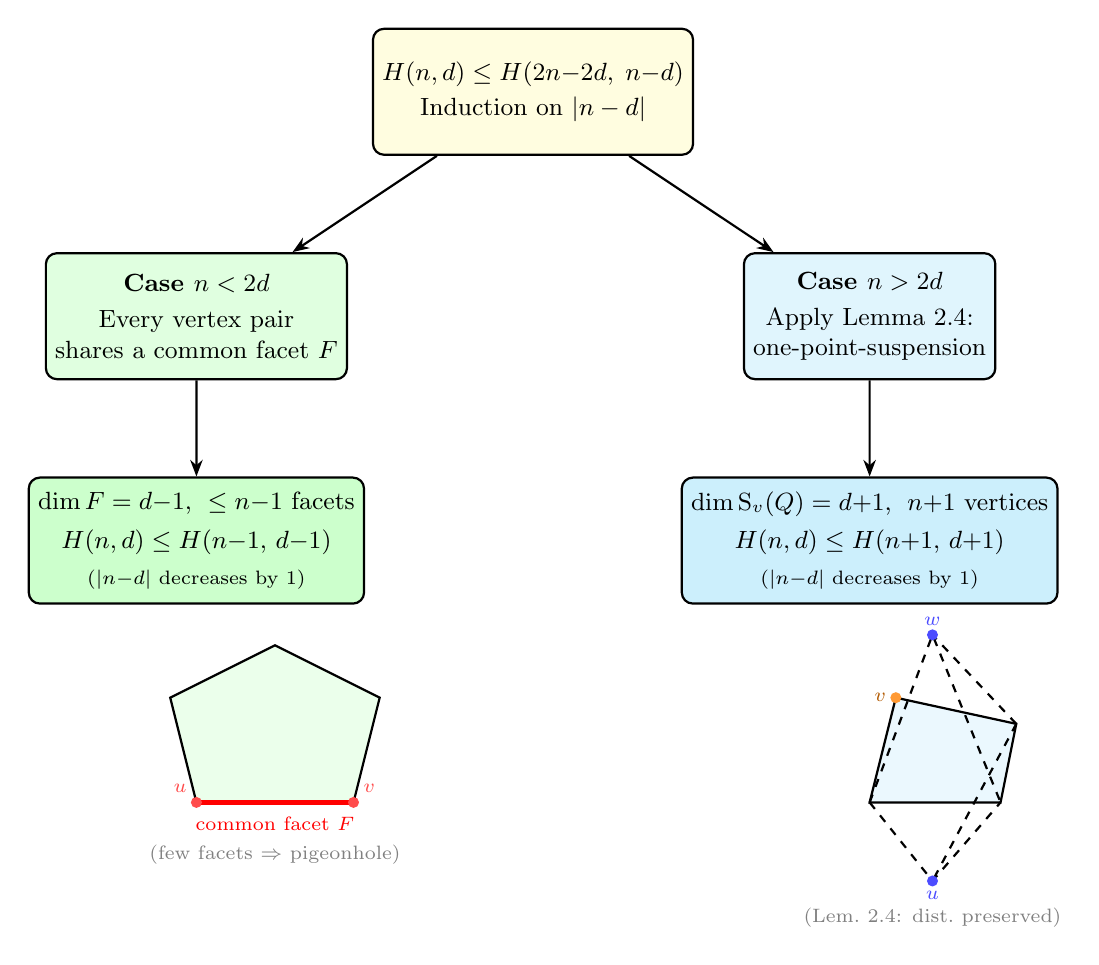
\begin{tikzpicture}[scale=0.95,
    box/.style={draw, thick, rounded corners=4pt, minimum width=3cm, minimum height=1.6cm, align=center, font=\small}]

  % Main statement
  \node[box, fill=yellow!12] (main) at (0,4) {$H(n,d) \leq H(2n{-}2d,\; n{-}d)$\\[2pt]
    Induction on $|n - d|$};

  % Case n < 2d
  \node[box, fill=green!12] (case1) at (-4.5,1) {\textbf{Case $n < 2d$}\\[2pt]
    Every vertex pair\\
    shares a common facet $F$};

  % Case n > 2d
  \node[box, fill=cyan!12] (case2) at (4.5,1) {\textbf{Case $n > 2d$}\\[2pt]
    Apply Lemma 2.4:\\
    one-point-suspension};

  % Results
  \node[box, fill=green!20] (res1) at (-4.5,-2) {$\dim F = d{-}1$,\;
    $\leq n{-}1$ facets\\[3pt]
    $H(n,d) \leq H(n{-}1,\, d{-}1)$\\[2pt]
    {\scriptsize ($|n{-}d|$ decreases by 1)}};

  \node[box, fill=cyan!20] (res2) at (4.5,-2) {$\dim \Sv(Q) = d{+}1$,\;
    $n{+}1$ vertices\\[3pt]
    $H(n,d) \leq H(n{+}1,\, d{+}1)$\\[2pt]
    {\scriptsize ($|n{-}d|$ decreases by 1)}};

  \draw[-{Stealth[length=6pt]}, thick] (main) -- (case1);
  \draw[-{Stealth[length=6pt]}, thick] (main) -- (case2);
  \draw[-{Stealth[length=6pt]}, thick] (case1) -- (res1);
  \draw[-{Stealth[length=6pt]}, thick] (case2) -- (res2);

  % Mini illustrations
  \begin{scope}[shift={(-4.5,-5.5)}, scale=0.7]
    \coordinate (a) at (0,0); \coordinate (b) at (3,0);
    \coordinate (c) at (3.5,2); \coordinate (d) at (1.5,3); \coordinate (e) at (-0.5,2);
    \fill[green!8] (a)--(b)--(c)--(d)--(e)--cycle;
    \draw[thick] (a)--(b)--(c)--(d)--(e)--cycle;
    \draw[ultra thick, red] (a)--(b);
    \node[font=\scriptsize, red] at (1.5,-0.4) {common facet $F$};
    \fill[red!70] (a) circle (3pt) node[above left, font=\scriptsize] {$u$};
    \fill[red!70] (b) circle (3pt) node[above right, font=\scriptsize] {$v$};
    \node[font=\scriptsize, gray] at (1.5,-1.0) {(few facets $\Rightarrow$ pigeonhole)};
  \end{scope}

  \begin{scope}[shift={(4.5,-5.5)}, scale=0.7]
    \coordinate (a) at (0,0); \coordinate (b) at (2.5,0);
    \coordinate (c) at (2.8,1.5); \coordinate (d) at (0.5,2);
    \fill[cyan!8] (a)--(b)--(c)--(d)--cycle;
    \draw[thick] (a)--(b)--(c)--(d)--cycle;
    \coordinate (u) at (1.2,-1.5); \coordinate (w) at (1.2,3.2);
    \draw[dashed, thick] (a)--(u)--(b); \draw[dashed, thick] (a)--(w)--(b);
    \draw[dashed, thick] (c)--(u); \draw[dashed, thick] (c)--(w);
    \fill[blue!70] (u) circle (3pt) node[below, font=\scriptsize] {$u$};
    \fill[blue!70] (w) circle (3pt) node[above, font=\scriptsize] {$w$};
    \fill[orange!80] (d) circle (3pt);
    \node[font=\scriptsize, orange!70!black, left] at (d) {$v$};
    \node[font=\scriptsize, gray] at (1.2,-2.2) {(Lem.\ 2.4: dist.\ preserved)};
  \end{scope}
\end{tikzpicture}
\caption*{\textbf{Proof of Lemma 1.1:}
Both cases decrease $|n - d|$ by 1, converging to the base case $n = 2d$
where the statement is tautological. \textbf{Put differently:}
$\max_{d}\{H(d+m, d)\} = H(2m, m)$ for all $m \in \mathbb{N}$.}
\end{figure}

\newpage

%% =============================================
%% THEOREM 2.6 — PARAGRAPH 1: Induction on asimpliciality
%% =============================================
\subsection*{Theorem 2.6 --- Strong $d$-step theorem for prismatoids}

\begin{figure}[h]
\centering
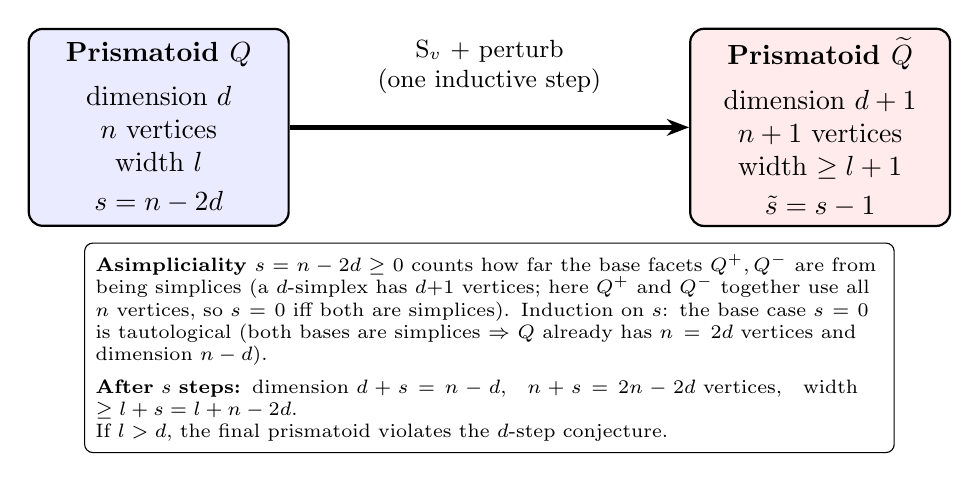
\begin{tikzpicture}[scale=1.0,
    pbox/.style={draw, thick, rounded corners=5pt, minimum width=3.3cm, minimum height=2.5cm, align=center}]

  \node[pbox, fill=blue!8] (Q) at (-4.2,0) {
    \textbf{Prismatoid $Q$}\\[4pt]
    dimension $d$\\
    $n$ vertices\\
    width $l$\\[2pt]
    $s = n - 2d$
  };

  \node[pbox, fill=red!8] (Qt) at (4.2,0) {
    \textbf{Prismatoid $\Qt$}\\[4pt]
    dimension $d+1$\\
    $n+1$ vertices\\
    width $\geq l+1$\\[2pt]
    $\tilde{s} = s - 1$
  };

  \draw[-{Stealth[length=8pt]}, ultra thick] (Q) -- (Qt)
    node[midway, above=8pt, font=\small, align=center] {$\Sv$ + perturb\\(one inductive step)};

  % Annotation: what s means
  \node[ann, text width=10cm] at (0,-2.8) {%
    \textbf{Asimpliciality} $s = n - 2d \geq 0$ counts how far
    the base facets $Q^+, Q^-$ are from being simplices (a $d$-simplex
    has $d{+}1$ vertices; here $Q^+$ and $Q^-$ together use all $n$ vertices, so
    $s = 0$ iff both are simplices).
    Induction on $s$: the base case $s = 0$ is tautological
    (both bases are simplices $\Rightarrow$ $Q$ already has $n = 2d$ vertices
    and dimension $n - d$).\\[4pt]
    \textbf{After $s$ steps:} dimension $d + s = n - d$, \;
    $n + s = 2n - 2d$ vertices, \;
    width $\geq l + s = l + n - 2d$.\\
    If $l > d$, the final prismatoid violates the $d$-step conjecture.
  };
\end{tikzpicture}
\caption*{\textbf{Theorem 2.6, paragraph 1 (induction setup):}
Each inductive step reduces asimpliciality by 1 while increasing dimension, vertices, and width each by 1.}
\end{figure}

%% =============================================
%% THEOREM 2.6 — PARAGRAPH 2: One-point-suspension
%% =============================================

\begin{figure}[h]
\centering
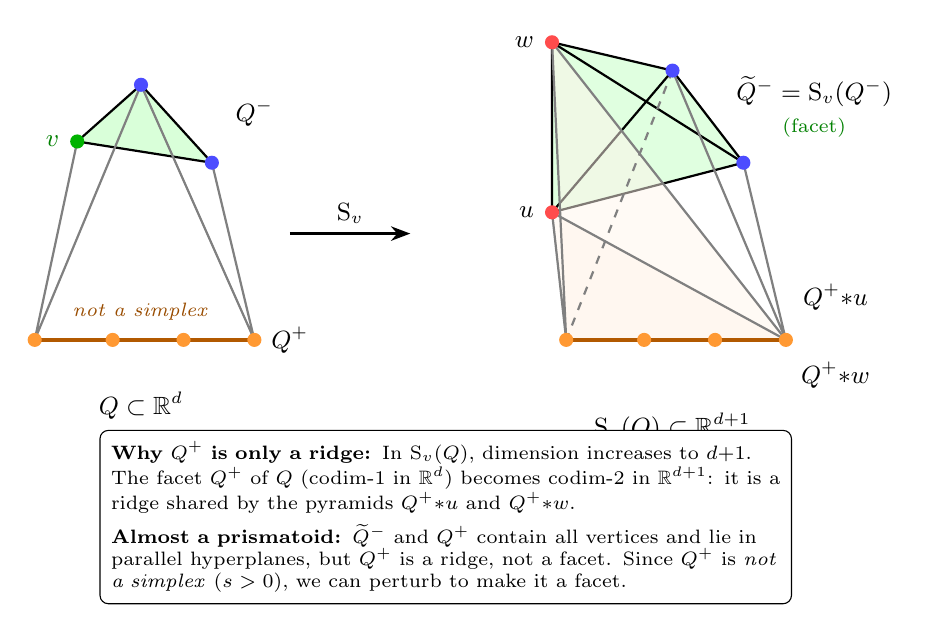
\begin{tikzpicture}[scale=0.9]
  %% --- Q (left) ---
  \begin{scope}[shift={(-5.5,0)}]
    % Q^- (simplex-like triangle at top)
    \coordinate (qm1) at (0.3,2.8);
    \coordinate (qm2) at (2.2,2.5);
    \coordinate (qm3) at (1.2,3.6);
    \fill[green!15] (qm1)--(qm2)--(qm3)--cycle;
    \draw[thick] (qm1)--(qm2)--(qm3)--cycle;
    \node[font=\small] at (2.8,3.2) {$Q^-$};

    % Q^+ (not a simplex: extra vertices on a line)
    \coordinate (qp1) at (-0.3,0);
    \coordinate (qp2) at (2.8,0);
    \coordinate (qp3) at (1.8,0);
    \coordinate (qp4) at (0.8,0);
    \draw[ultra thick, orange!70!black] (qp1)--(qp2);
    \node[font=\small] at (3.3,0) {$Q^+$};
    \node[font=\scriptsize, orange!60!black] at (1.2,0.4) {\emph{not a simplex}};

    % Connecting edges
    \draw[thick, gray] (qp1)--(qm1) (qp1)--(qm3) (qp2)--(qm2) (qp2)--(qm3);

    % Vertices
    \foreach \p in {qm2,qm3} \node[vtx] at (\p) {};
    \node[vtx, fill=green!70!black] at (qm1) {};
    \node[left=3pt, font=\small, green!50!black] at (qm1) {$v$};
    \foreach \p in {qp1,qp2,qp3,qp4} \node[vtx, fill=orange!80] at (\p) {};

    \node[font=\small, below] at (1.2,-0.6) {$Q \subset \mathbb{R}^d$};
  \end{scope}

  \draw[-{Stealth[length=7pt]}, thick] (-2.2,1.5) -- (-0.5,1.5)
    node[midway, above, font=\small] {$\Sv$};

  %% --- S_v(Q) (right) ---
  \begin{scope}[shift={(2,0)}]
    % S_v(Q^-) = tilde{Q}^-
    \coordinate (sqm2) at (2.2,2.5);
    \coordinate (sqm3) at (1.2,3.8);
    \coordinate (u) at (-0.5,1.8);
    \coordinate (w) at (-0.5,4.2);

    \fill[green!12] (u)--(sqm2)--(sqm3)--(w)--cycle;
    \draw[thick] (u)--(sqm2)--(sqm3)--(w)--cycle;
    \draw[thick] (u)--(sqm3) (w)--(sqm2);
    \node[font=\small] at (3.2,3.5) {$\Qt^- = \Sv(Q^-)$};
    \node[font=\scriptsize, green!50!black] at (3.2,3.0) {(facet)};

    % Q^+ as a ridge
    \coordinate (qp1) at (-0.3,0);
    \coordinate (qp2) at (2.8,0);
    \coordinate (qp3) at (1.8,0);
    \coordinate (qp4) at (0.8,0);

    % Pyramids Q^+ * u and Q^+ * w
    \fill[orange!8, opacity=0.5] (qp1)--(qp2)--(u)--cycle;
    \fill[orange!8, opacity=0.5] (qp1)--(qp2)--(w)--cycle;
    \draw[thick, gray] (qp1)--(u)--(qp2) (qp1)--(w)--(qp2);
    \draw[ultra thick, orange!70!black] (qp1)--(qp2);

    % Connecting edges
    \draw[thick, gray] (sqm2)--(qp2) (sqm3)--(qp2);
    \draw[thick, gray, dashed] (sqm3)--(qp1);

    % Vertices
    \foreach \p in {sqm2,sqm3} \node[vtx] at (\p) {};
    \node[svtx] at (u) {};
    \node[svtx] at (w) {};
    \node[left=3pt, font=\small] at (u) {$u$};
    \node[left=3pt, font=\small] at (w) {$w$};
    \foreach \p in {qp1,qp2,qp3,qp4} \node[vtx, fill=orange!80] at (\p) {};

    \node[font=\small] at (3.5,0.6) {$Q^+{\ast}u$};
    \node[font=\small] at (3.5,-0.5) {$Q^+{\ast}w$};

    \node[font=\small, below] at (1.2,-0.9) {$\Sv(Q) \subset \mathbb{R}^{d+1}$};
  \end{scope}

  % Key proof point annotation
  \node[ann, text width=8.5cm] at (0,-2.5) {%
    \textbf{Why $Q^+$ is only a ridge:} In $\Sv(Q)$, dimension increases to
    $d{+}1$. The facet $Q^+$ of $Q$ (codim-1 in $\mathbb{R}^d$) becomes codim-2
    in $\mathbb{R}^{d+1}$: it is a ridge shared by the pyramids $Q^+{\ast}u$ and $Q^+{\ast}w$.\\[3pt]
    \textbf{Almost a prismatoid:} $\Qt^-$ and $Q^+$ contain all vertices and lie
    in parallel hyperplanes, but $Q^+$ is a ridge, not a facet.
    Since $Q^+$ is \emph{not a simplex} ($s > 0$), we can perturb to make it a facet.
  };
\end{tikzpicture}
\caption*{\textbf{Theorem 2.6, paragraph 2:}
The one-point-suspension $\Sv(Q)$ replaces $v \in Q^-$ with two new vertices $u, w$
on opposite sides, with $v$ on segment $uw$. The facet $Q^-$ becomes $\Qt^- = \Sv(Q^-)$.
The former facet $Q^+$ is now only a ridge.}
\end{figure}

\newpage

%% =============================================
%% THEOREM 2.6 — PARAGRAPH 3: The perturbation
%% =============================================

\begin{figure}[h]
\centering
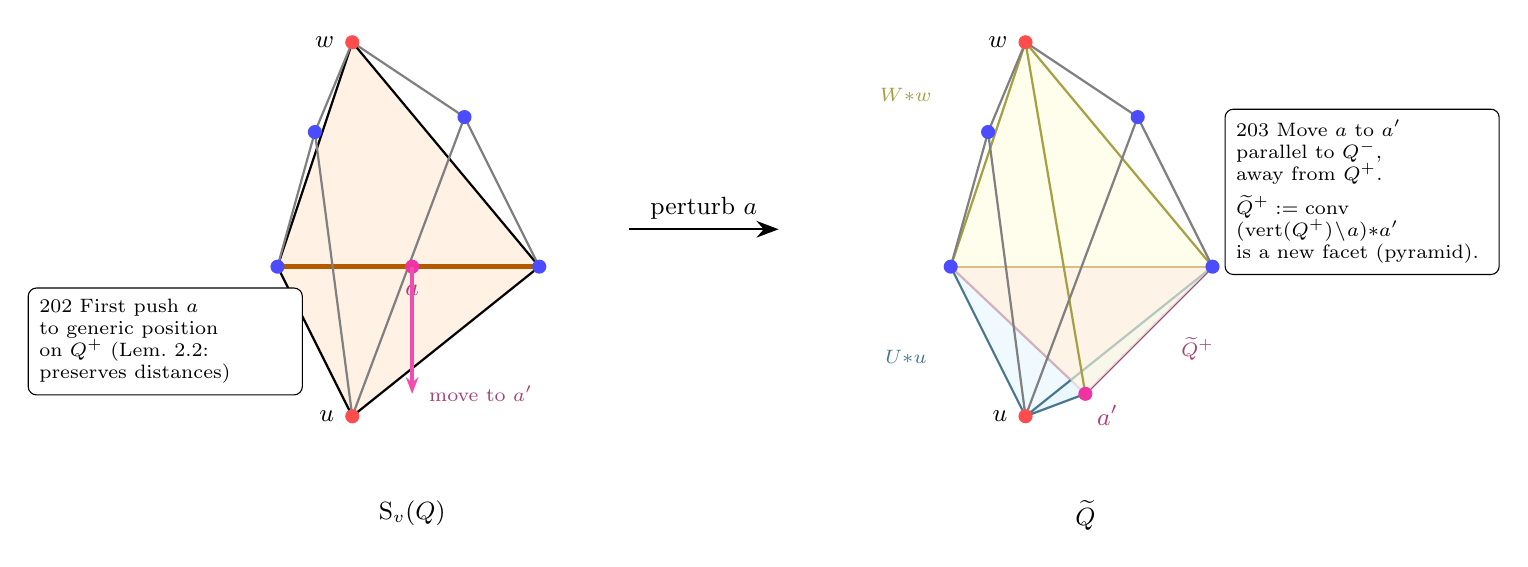
\begin{tikzpicture}[scale=0.95]
  %% S_v(Q) before perturbation (left)
  \begin{scope}[shift={(-5,0)}]
    \coordinate (u) at (0,-1.5);
    \coordinate (w) at (0,3.5);
    \coordinate (p1) at (-1,0.5);
    \coordinate (p2) at (2.5,0.5);
    \coordinate (a) at (0.8,0.5);
    \coordinate (qm1) at (1.5,2.5);
    \coordinate (qm2) at (-0.5,2.3);

    % Q+ * u and Q+ * w
    \fill[orange!10] (p1)--(p2)--(u)--cycle;
    \fill[orange!10] (p1)--(p2)--(w)--cycle;
    \draw[thick] (p1)--(u)--(p2) (p1)--(w)--(p2);
    \draw[ultra thick, orange!70!black] (p1)--(p2);

    % Other edges
    \draw[thick, gray] (u)--(qm1)--(w) (u)--(qm2)--(w);
    \draw[thick, gray] (qm1)--(p2) (qm2)--(p1);

    % Vertices
    \node[svtx] at (u) {}; \node[svtx] at (w) {};
    \node[left=3pt, font=\small] at (u) {$u$};
    \node[left=3pt, font=\small] at (w) {$w$};
    \foreach \p in {p1,p2,qm1,qm2} \node[vtx] at (\p) {};
    \node[pvtx] at (a) {};
    \node[below=3pt, font=\small, magenta!70!black] at (a) {$a$};

    % Move arrow
    \draw[-{Stealth[length=6pt]}, ultra thick, magenta!70] (a) -- ++(0,-1.7)
      node[right=2pt, font=\scriptsize, magenta!60!black] {move to $a'$};

    \node[font=\small, below] at (0.8,-2.5) {$\Sv(Q)$};

    % Step labels
    \node[ann, text width=3.2cm] at (-2.5,-0.5) {\scriptsize
      \ding{202} First push $a$\\
      to generic position\\
      on $Q^+$ (Lem.\ 2.2:\\
      preserves distances)};
  \end{scope}

  \draw[-{Stealth[length=8pt]}, thick] (-1.3,1) -- (0.7,1)
    node[midway, above, font=\small] {perturb $a$};

  %% \tilde{Q} after perturbation (right)
  \begin{scope}[shift={(4,0)}]
    \coordinate (u) at (0,-1.5);
    \coordinate (w) at (0,3.5);
    \coordinate (p1) at (-1,0.5);
    \coordinate (p2) at (2.5,0.5);
    \coordinate (aprime) at (0.8,-1.2);
    \coordinate (qm1) at (1.5,2.5);
    \coordinate (qm2) at (-0.5,2.3);

    % \tilde{Q}^+ = pyramid over (Q+ \ a) with apex a'
    \fill[magenta!10] (p1)--(p2)--(aprime)--cycle;
    \draw[thick, magenta!60!black] (p1)--(aprime)--(p2);
    \draw[thick, orange!70!black] (p1)--(p2);
    \node[font=\scriptsize, magenta!60!black] at (2.3,-0.6) {$\Qt^+$};

    % U*u (lower envelope pyramided with u)
    \fill[cyan!10, opacity=0.6] (p1)--(aprime)--(u)--cycle;
    \fill[cyan!10, opacity=0.6] (aprime)--(p2)--(u)--cycle;
    \draw[thick, cyan!50!black] (p1)--(u)--(aprime) (aprime)--(u)--(p2);

    % W*w (upper envelope pyramided with w)
    \fill[yellow!12, opacity=0.6] (p1)--(aprime)--(w)--cycle;
    \fill[yellow!12, opacity=0.6] (aprime)--(p2)--(w)--cycle;
    \draw[thick, yellow!60!black] (p1)--(w)--(aprime) (aprime)--(w)--(p2);

    % Other edges
    \draw[thick, gray] (u)--(qm1)--(w) (u)--(qm2)--(w);
    \draw[thick, gray] (qm1)--(p2) (qm2)--(p1);

    \node[svtx] at (u) {}; \node[svtx] at (w) {};
    \node[left=3pt, font=\small] at (u) {$u$};
    \node[left=3pt, font=\small] at (w) {$w$};
    \foreach \p in {p1,p2,qm1,qm2} \node[vtx] at (\p) {};
    \node[pvtx] at (aprime) {};
    \node[below right=1pt, font=\small, magenta!70!black] at (aprime) {$a'$};

    \node[font=\scriptsize, cyan!50!black] at (-1.6,-0.7) {$U{\ast}u$};
    \node[font=\scriptsize, yellow!60!black] at (-1.6,2.8) {$W{\ast}w$};

    \node[font=\small, below] at (0.8,-2.5) {$\Qt$};

    % Step label
    \node[ann, text width=3.2cm] at (4.5,1.5) {\scriptsize
      \ding{203} Move $a$ to $a'$\\
      parallel to $Q^-$,\\
      away from $Q^+$.\\[3pt]
      $\Qt^+ := \mathrm{conv}$\\
      $(\mathrm{vert}(Q^+)\!\setminus\! a){\ast}a'$\\
      is a new facet (pyramid).};
  \end{scope}
\end{tikzpicture}
\caption*{\textbf{Theorem 2.6, paragraph 3 (the perturbation):}
The vertex $a \in Q^+$ is first pushed to a generic position (using Lemma 2.2, which
preserves dual distances). Then $a$ is moved to $a'$, creating the new base facet $\Qt^+$.
The old pyramid facets $Q^+{\ast}u$ and $Q^+{\ast}w$ are each refined: the lower and upper
envelopes of $\Qt^+$ yield complexes $U$ and $W$, giving facets $U{\ast}u$ and $W{\ast}w$.}
\end{figure}


%% =============================================
%% THEOREM 2.6 — PARAGRAPH 4: Width argument
%% =============================================

\begin{figure}[h]
\centering
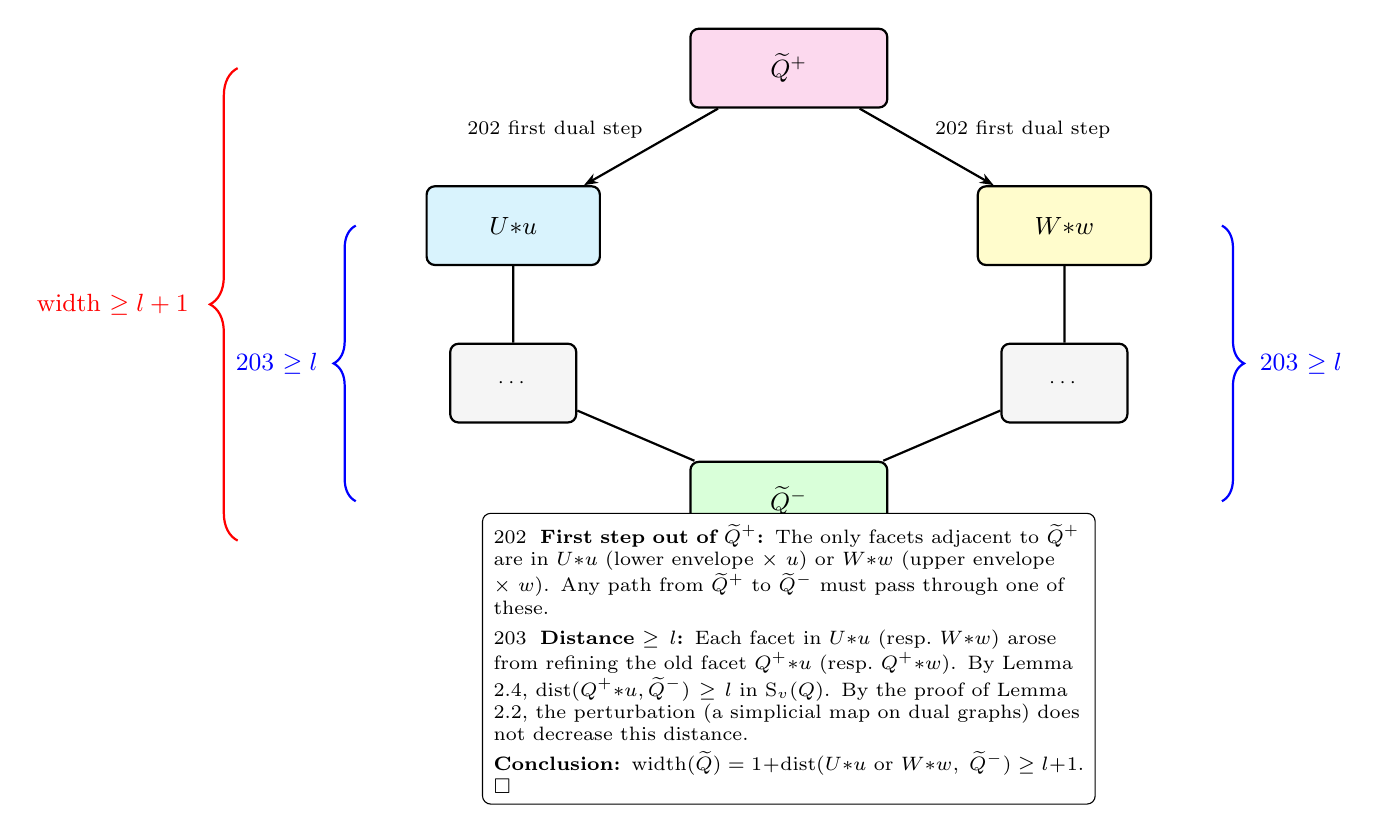
\begin{tikzpicture}[scale=1.0]
  % Central facet Q~+
  \node[fbox, fill=magenta!15, minimum width=2.5cm] (Qtp) at (0,0.5) {$\Qt^+$};

  % U*u and W*w
  \node[fbox, fill=cyan!15, minimum width=2.2cm] (Uu) at (-3.5,-1.5) {$U{\ast}u$};
  \node[fbox, fill=yellow!20, minimum width=2.2cm] (Ww) at (3.5,-1.5) {$W{\ast}w$};

  % \tilde{Q}^- at bottom
  \node[fbox, fill=green!15, minimum width=2.5cm] (Qtm) at (0,-5) {$\Qt^-$};

  % Intermediate
  \node[fbox, fill=gray!8, minimum width=1.6cm, font=\scriptsize] (oth1) at (-3.5,-3.5) {$\cdots$};
  \node[fbox, fill=gray!8, minimum width=1.6cm, font=\scriptsize] (oth2) at (3.5,-3.5) {$\cdots$};

  % First step from Q~+
  \draw[-{Stealth[length=5pt]}, thick] (Qtp) -- (Uu)
    node[midway, above left=-1pt, font=\scriptsize] {\ding{202} first dual step};
  \draw[-{Stealth[length=5pt]}, thick] (Qtp) -- (Ww)
    node[midway, above right=-1pt, font=\scriptsize] {\ding{202} first dual step};

  % Path to Q~-
  \draw[thick] (Uu) -- (oth1) -- (Qtm);
  \draw[thick] (Ww) -- (oth2) -- (Qtm);

  % Distance braces
  \draw[decorate, decoration={brace, amplitude=8pt, mirror}, thick, blue]
    (-5.5,-1.5) -- (-5.5,-5) node[midway, left=10pt, font=\small, blue, align=center]
    {\ding{203} $\geq l$};

  \draw[decorate, decoration={brace, amplitude=8pt}, thick, blue]
    (5.5,-1.5) -- (5.5,-5) node[midway, right=10pt, font=\small, blue, align=center]
    {\ding{203} $\geq l$};

  % Total width brace
  \draw[decorate, decoration={brace, amplitude=10pt, mirror}, thick, red]
    (-7,0.5) -- (-7,-5.5) node[midway, left=14pt, font=\small, red, align=center]
    {width $\geq l + 1$};

  % Proof annotations
  \node[ann, text width=7.5cm] at (0,-7) {%
    \ding{202}\; \textbf{First step out of $\Qt^+$:}
    The only facets adjacent to $\Qt^+$ are in $U{\ast}u$ (lower envelope $\times$ $u$)
    or $W{\ast}w$ (upper envelope $\times$ $w$). Any path from $\Qt^+$ to $\Qt^-$ must
    pass through one of these.\\[3pt]
    \ding{203}\; \textbf{Distance $\geq l$:}
    Each facet in $U{\ast}u$ (resp.\ $W{\ast}w$) arose from refining the old
    facet $Q^+{\ast}u$ (resp.\ $Q^+{\ast}w$).
    By Lemma 2.4, $\mathrm{dist}(Q^+{\ast}u, \Qt^-) \geq l$ in $\Sv(Q)$.
    By the proof of Lemma 2.2, the perturbation (a simplicial map on dual graphs)
    does not decrease this distance.\\[3pt]
    \textbf{Conclusion:}
    $\mathrm{width}(\Qt) = 1 + \mathrm{dist}(U{\ast}u \text{ or } W{\ast}w,\; \Qt^-) \geq l + 1$.\quad$\square$
  };
\end{tikzpicture}
\caption*{\textbf{Theorem 2.6, paragraph 4 (width argument):}
The width increases by at least 1 because leaving $\Qt^+$ costs one step,
and then you are still at distance $\geq l$ from $\Qt^-$.}
\end{figure}

\newpage

%% =============================================
%% OCTAHEDRON FACET ADJACENCY (Figure 4 style)
%% =============================================
\subsection*{Facet adjacency of the octahedron as a prismatoid (cf.\ Figure 4)}

The regular octahedron with vertices $V_1{=}(\pm1,0,0)$, $V_3{=}(0,\pm1,0)$,
$V_5{=}(0,0,\pm1)$ is a prismatoid with base facets
$Q^+ = \{V_1, V_3, V_5\}$ (in the plane $x_1{+}x_2{+}x_3 = 1$) and
$Q^- = \{V_2, V_4, V_6\}$ (in $x_1{+}x_2{+}x_3 = -1$), where
$V_2 = -V_1$, $V_4 = -V_3$, $V_6 = -V_5$.
It has $d = 3$, $n = 6$, and width $l = 3 = d$ (the $d$-step bound is tight).

\begin{figure}[h]
\centering
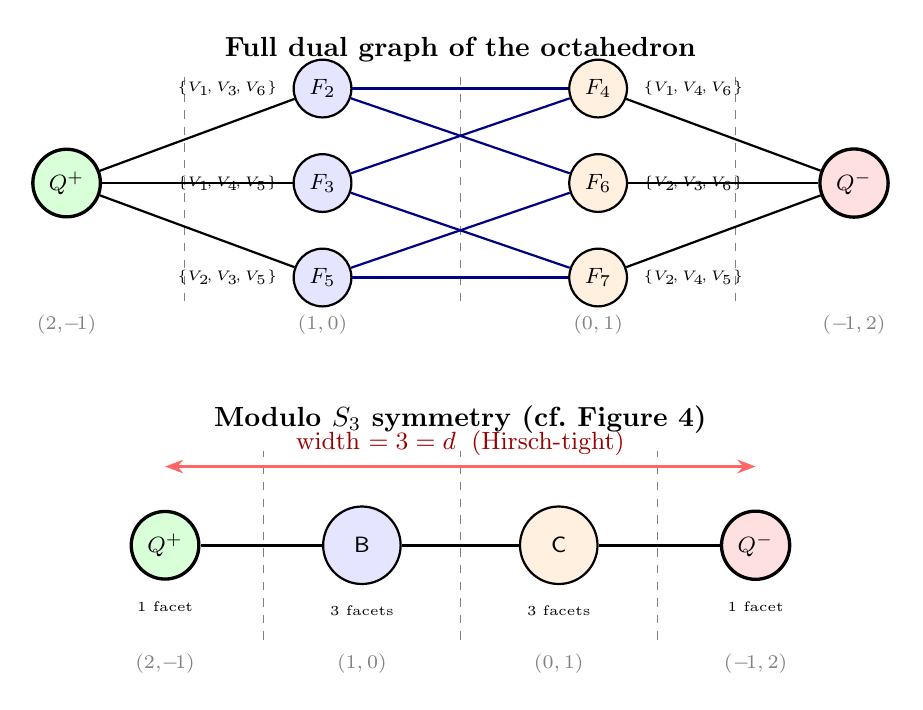
\begin{tikzpicture}[scale=1.0,
    fnode/.style={circle, draw, thick, minimum size=20pt, font=\footnotesize},
    bnode/.style={circle, draw, thick, minimum size=22pt, font=\footnotesize, very thick}]

  %% ============================================
  %% FULL ADJACENCY GRAPH (top)
  %% ============================================
  \node[font=\bfseries] at (5,7.5) {Full dual graph of the octahedron};

  % Dashed vertical separators
  \draw[dashed, gray] (1.5,4.3) -- (1.5,7.2);
  \draw[dashed, gray] (5,4.3) -- (5,7.2);
  \draw[dashed, gray] (8.5,4.3) -- (8.5,7.2);

  % Bidimension labels
  \node[font=\scriptsize, gray] at (0,4.0) {$(2,\!-\!1)$};
  \node[font=\scriptsize, gray] at (3.25,4.0) {$(1,0)$};
  \node[font=\scriptsize, gray] at (6.75,4.0) {$(0,1)$};
  \node[font=\scriptsize, gray] at (10,4.0) {$(-\!1,2)$};

  % Q+ node
  \node[bnode, fill=green!15] (Qp) at (0,5.8) {$Q^+$};

  % (1,0) nodes — each shares an edge of Q+ with Q+, plus one vertex of Q-
  \node[fnode, fill=blue!10] (F2) at (3.25,7) {$F_2$};
  \node[fnode, fill=blue!10] (F3) at (3.25,5.8) {$F_3$};
  \node[fnode, fill=blue!10] (F5) at (3.25,4.6) {$F_5$};

  % (0,1) nodes — each has one vertex of Q+, plus an edge of Q-
  \node[fnode, fill=orange!12] (F4) at (6.75,7) {$F_4$};
  \node[fnode, fill=orange!12] (F6) at (6.75,5.8) {$F_6$};
  \node[fnode, fill=orange!12] (F7) at (6.75,4.6) {$F_7$};

  % Q- node
  \node[bnode, fill=red!12] (Qm) at (10,5.8) {$Q^-$};

  % Q+ to (1,0) edges
  \draw[thick] (Qp) -- (F2);
  \draw[thick] (Qp) -- (F3);
  \draw[thick] (Qp) -- (F5);

  % (0,1) to Q- edges
  \draw[thick] (F4) -- (Qm);
  \draw[thick] (F6) -- (Qm);
  \draw[thick] (F7) -- (Qm);

  % Cross adjacencies (1,0) -- (0,1): each connects to 2 of 3
  % F2 -- F4, F6 (not F7)
  \draw[thick, blue!50!black] (F2) -- (F4);
  \draw[thick, blue!50!black] (F2) -- (F6);
  % F3 -- F4, F7 (not F6)
  \draw[thick, blue!50!black] (F3) -- (F4);
  \draw[thick, blue!50!black] (F3) -- (F7);
  % F5 -- F6, F7 (not F4)
  \draw[thick, blue!50!black] (F5) -- (F6);
  \draw[thick, blue!50!black] (F5) -- (F7);

  % Vertex labels — outside the graph
  \node[font=\tiny, left=2pt, align=right] at (F2.west) {$\{V_1\!,V_3\!,V_6\}$};
  \node[font=\tiny, left=2pt, align=right] at (F3.west) {$\{V_1\!,V_4\!,V_5\}$};
  \node[font=\tiny, left=2pt, align=right] at (F5.west) {$\{V_2\!,V_3\!,V_5\}$};
  \node[font=\tiny, right=2pt, align=left] at (F4.east) {$\{V_1\!,V_4\!,V_6\}$};
  \node[font=\tiny, right=2pt, align=left] at (F6.east) {$\{V_2\!,V_3\!,V_6\}$};
  \node[font=\tiny, right=2pt, align=left] at (F7.east) {$\{V_2\!,V_4\!,V_5\}$};

  %% ============================================
  %% MODULO SYMMETRY (bottom) — Figure 4 style
  %% ============================================
  \node[font=\bfseries] at (5,2.8) {Modulo $S_3$ symmetry (cf.\ Figure 4)};

  % Dashed vertical separators
  \draw[dashed, gray] (2.5,0) -- (2.5,2.4);
  \draw[dashed, gray] (5,0) -- (5,2.4);
  \draw[dashed, gray] (7.5,0) -- (7.5,2.4);

  % Bidimension labels below
  \node[font=\scriptsize, gray] at (1.25,-0.3) {$(2,\!-\!1)$};
  \node[font=\scriptsize, gray] at (3.75,-0.3) {$(1,0)$};
  \node[font=\scriptsize, gray] at (6.25,-0.3) {$(0,1)$};
  \node[font=\scriptsize, gray] at (8.75,-0.3) {$(-\!1,2)$};

  % Nodes
  \node[bnode, fill=green!15] (A) at (1.25,1.2) {$Q^+$};
  \node[fnode, fill=blue!10, minimum size=28pt] (B) at (3.75,1.2) {\textsf{B}};
  \node[fnode, fill=orange!12, minimum size=28pt] (C) at (6.25,1.2) {\textsf{C}};
  \node[bnode, fill=red!12] (L) at (8.75,1.2) {$Q^-$};

  % Edges
  \draw[very thick] (A) -- (B);
  \draw[very thick] (B) -- (C);
  \draw[very thick] (C) -- (L);

  % Orbit sizes
  \node[font=\tiny, below=4pt] at (A.south) {1 facet};
  \node[font=\tiny, below=4pt] at (B.south) {3 facets};
  \node[font=\tiny, below=4pt] at (C.south) {3 facets};
  \node[font=\tiny, below=4pt] at (L.south) {1 facet};

  % Width annotation
  \draw[{Stealth}-{Stealth}, thick, red!60] (1.25,2.2) -- (8.75,2.2)
    node[midway, above, font=\small, red!60!black] {width $= 3 = d$ \;(Hirsch-tight)};
\end{tikzpicture}
\caption*{\textbf{Facet adjacency of the octahedron (prismatoid with opposite triangular bases).}
\emph{Top:} The full dual graph. $Q^+$ is adjacent only to the three bidimension-$(1,0)$ facets;
each $(1,0)$ facet is adjacent to exactly 2 of the 3 $(0,1)$ facets (the cross-edges form $K_{3,3}$
minus a perfect matching); $Q^-$ is adjacent only to the $(0,1)$ facets.
\emph{Bottom:} Modulo the $S_3$ symmetry (permuting coordinate axes), there are 4 orbits.
The width is $3 = d$: the $d$-step conjecture bound is tight.
Bidimension $(i,j)$ means the facet is the convex hull of an $i$-face of $Q^+$
and a $j$-face of $Q^-$ (the empty face has dimension $-1$).}
\end{figure}

\newpage

%% =============================================
%% OCTAHEDRON: Q+, Q-, and Minkowski sum
%% =============================================
\subsection*{The octahedron as a prismatoid: $Q^+$, $Q^-$, and $Q^+ + Q^-$}

The cross-section of the octahedron at height $t \in [-1,1]$ is
$\tfrac{1+t}{2}\,Q^+ + \tfrac{1-t}{2}\,Q^-$.
At $t=0$ this is $\tfrac{1}{2}(Q^+ + Q^-)$, a regular hexagon.
The Minkowski sum of two triangles pointing in opposite directions always yields a hexagon.

\begin{figure}[h]
\centering
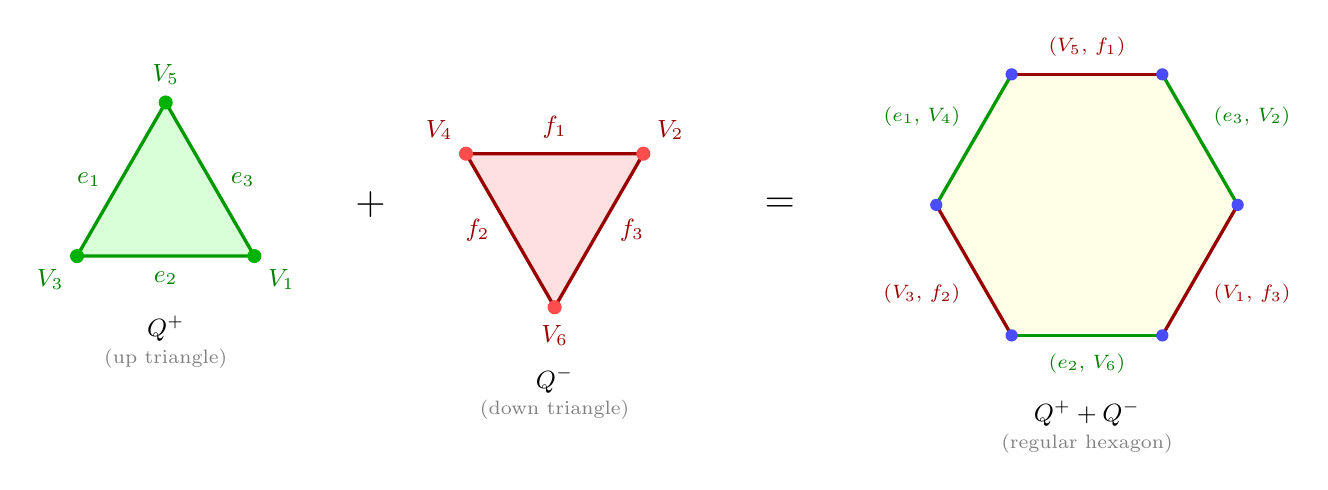
\begin{tikzpicture}[scale=1.3]

  %% ==================
  %% Q+ (up triangle)
  %% ==================
  \begin{scope}[shift={(-4.8,0)}]
    \coordinate (A) at (0, 1);
    \coordinate (B) at (-0.866, -0.5);
    \coordinate (C) at (0.866, -0.5);

    \fill[green!15] (A)--(B)--(C)--cycle;
    \draw[very thick, green!60!black] (A)--(B)--(C)--cycle;

    \node[vtx, fill=green!70!black] at (A) {};
    \node[vtx, fill=green!70!black] at (B) {};
    \node[vtx, fill=green!70!black] at (C) {};

    \node[above=3pt, font=\small, green!50!black] at (A) {$V_5$};
    \node[below left=2pt, font=\small, green!50!black] at (B) {$V_3$};
    \node[below right=2pt, font=\small, green!50!black] at (C) {$V_1$};

    % Edge (facet) labels
    \node[font=\small, green!50!black, left=4pt] at (-0.433, 0.25) {$e_1$};
    \node[font=\small, green!50!black, below=2pt] at (0, -0.5) {$e_2$};
    \node[font=\small, green!50!black, right=4pt] at (0.433, 0.25) {$e_3$};

    \node[below=18pt, font=\small] at (0,-0.5) {$Q^+$};
    \node[below=30pt, font=\scriptsize, gray] at (0,-0.5) {(up triangle)};
  \end{scope}

  % Plus sign
  \node[font=\Large] at (-2.8,0) {$+$};

  %% ==================
  %% Q- (down triangle)
  %% ==================
  \begin{scope}[shift={(-1,0)}]
    \coordinate (D) at (0, -1);
    \coordinate (E) at (0.866, 0.5);
    \coordinate (F) at (-0.866, 0.5);

    \fill[red!12] (D)--(E)--(F)--cycle;
    \draw[very thick, red!60!black] (D)--(E)--(F)--cycle;

    \node[vtx, fill=red!70] at (D) {};
    \node[vtx, fill=red!70] at (E) {};
    \node[vtx, fill=red!70] at (F) {};

    \node[below=3pt, font=\small, red!60!black] at (D) {$V_6$};
    \node[above right=2pt, font=\small, red!60!black] at (E) {$V_2$};
    \node[above left=2pt, font=\small, red!60!black] at (F) {$V_4$};

    % Edge (facet) labels
    \node[font=\small, red!60!black, above=2pt] at (0, 0.5) {$f_1$};
    \node[font=\small, red!60!black, left=4pt] at (-0.433, -0.25) {$f_2$};
    \node[font=\small, red!60!black, right=4pt] at (0.433, -0.25) {$f_3$};

    \node[below=18pt, font=\small] at (0,-1) {$Q^-$};
    \node[below=30pt, font=\scriptsize, gray] at (0,-1) {(down triangle)};
  \end{scope}

  % Equals sign
  \node[font=\Large] at (1.2,0) {$=$};

  %% ==========================
  %% Minkowski sum (hexagon)
  %% ==========================
  \begin{scope}[shift={(4.2,0)}, scale=0.85]
    % Hexagon vertices = Q+ vertex + Q- vertex
    \coordinate (H1) at (0.866, 1.5);    % A+E = V5+V2
    \coordinate (H2) at (-0.866, 1.5);   % A+F = V5+V4
    \coordinate (H3) at (-1.732, 0);     % B+F = V3+V4
    \coordinate (H4) at (-0.866, -1.5);  % B+D = V3+V6
    \coordinate (H5) at (0.866, -1.5);   % C+D = V1+V6
    \coordinate (H6) at (1.732, 0);      % C+E = V1+V2

    % Fill
    \fill[yellow!10] (H1)--(H2)--(H3)--(H4)--(H5)--(H6)--cycle;

    % Hexagon edges — alternating Q- (orange) and Q+ (green) contributions
    % Top: H1→H2, parallel to Q- edge E→F
    \draw[very thick, red!60!black] (H1)--(H2);
    % Upper-left: H2→H3, parallel to Q+ edge A→B
    \draw[very thick, green!60!black] (H2)--(H3);
    % Lower-left: H3→H4, parallel to Q- edge F→D
    \draw[very thick, red!60!black] (H3)--(H4);
    % Bottom: H4→H5, parallel to Q+ edge B→C
    \draw[very thick, green!60!black] (H4)--(H5);
    % Lower-right: H5→H6, parallel to Q- edge D→E
    \draw[very thick, red!60!black] (H5)--(H6);
    % Upper-right: H6→H1, parallel to Q+ edge C→A
    \draw[very thick, green!60!black] (H6)--(H1);

    % Vertex dots and labels
    \foreach \h in {H1,H2,H3,H4,H5,H6}
      \fill[blue!70] (\h) circle (2pt);

    % Facet labels as (face of Q+, face of Q-)
    \node[font=\scriptsize, red!60!black, above=3pt] at ($(H1)!0.5!(H2)$) {$(V_5,\, f_1)$};
    \node[font=\scriptsize, green!50!black, above left=2pt] at ($(H2)!0.5!(H3)$) {$(e_1,\, V_4)$};
    \node[font=\scriptsize, red!60!black, below left=2pt] at ($(H3)!0.5!(H4)$) {$(V_3,\, f_2)$};
    \node[font=\scriptsize, green!50!black, below=3pt] at ($(H4)!0.5!(H5)$) {$(e_2,\, V_6)$};
    \node[font=\scriptsize, red!60!black, below right=2pt] at ($(H5)!0.5!(H6)$) {$(V_1,\, f_3)$};
    \node[font=\scriptsize, green!50!black, above right=2pt] at ($(H6)!0.5!(H1)$) {$(e_3,\, V_2)$};

    \node[below=20pt, font=\small] at (0,-1.5) {$Q^+ + Q^-$};
    \node[below=32pt, font=\scriptsize, gray] at (0,-1.5) {(regular hexagon)};

  \end{scope}
\end{tikzpicture}
\caption*{\textbf{Minkowski sum of the base facets.}
$Q^+$ has edges $e_1 = V_3 V_5$, $e_2 = V_1 V_3$, $e_3 = V_1 V_5$;
$Q^-$ has edges $f_1 = V_2 V_4$, $f_2 = V_4 V_6$, $f_3 = V_2 V_6$.
Their Minkowski sum is a regular hexagon whose 6 edges alternate between translates
of $Q^+$ edges (\textcolor{green!60!black}{green}) and $Q^-$ edges
(\textcolor{red!60!black}{red}).
Each edge of the hexagon corresponds to a non-base facet of the octahedron,
labeled by its pair of faces: $(e_i, V_j)$ for the $(1,0)$ facets
and $(V_i, f_j)$ for the $(0,1)$ facets.}
\end{figure}

\end{document}
